\documentclass[11pt]{article}

% --- Silnik: xelatex ---
\usepackage{fontspec}
\setmainfont{DejaVu Serif}[Scale=0.94]
\setsansfont{DejaVu Sans}[Scale=0.94]
\setmonofont{DejaVu Sans Mono}[Scale=0.86]

\usepackage{amssymb}
\usepackage[a4paper,margin=2.3cm]{geometry}
\usepackage{xcolor}
\usepackage{titlesec}
\usepackage{enumitem}
\usepackage{booktabs}
\usepackage{tabularx}
\usepackage{array}
\usepackage{tikz}

\definecolor{navy}{RGB}{19,40,82}
\definecolor{rulegrey}{RGB}{180,190,205}
\definecolor{accent}{RGB}{0,110,90}

\emergencystretch=3em
\hbadness=2500

\titleformat{\section}{\Large\bfseries\sffamily\color{navy}}{}{0pt}{}
\titleformat{\subsection}{\large\bfseries\sffamily\color{navy}}{}{0pt}{}
\titleformat{\subsubsection}{\normalsize\bfseries\sffamily\color{navy}}{}{0pt}{}
\titlespacing*{\section}{0pt}{1.25em}{0.4em}
\titlespacing*{\subsection}{0pt}{0.85em}{0.2em}
\titlespacing*{\subsubsection}{0pt}{0.6em}{0.15em}

\setlength{\parindent}{0pt}
\setlength{\parskip}{0.5em}
\setlist[itemize]{leftmargin=1.3em,itemsep=0.12em,topsep=0.2em}
\setlist[enumerate]{leftmargin=1.5em,itemsep=0.12em,topsep=0.2em}

\newcommand{\ra}{$\rightarrow$}
\newcommand{\key}[1]{\textbf{\color{navy}#1}}

\begin{document}

% ====== TYTUL ======
{\sffamily\bfseries\color{navy}\LARGE Projekt: Cyfrowy bliźniak i testbench diagnostyczny ładowarek AC}\\[3pt]
{\sffamily\large\color{navy} Model-based diagnostyka, weryfikacja licznika i raporty do producenta}\\[5pt]
{\color{rulegrey}\rule{\linewidth}{1pt}}\\[3pt]
{\sffamily\small Dawid Cekała \quad$\cdot$\quad zadanie rekrutacyjne AMPERE POINT --- część 2 \quad$\cdot$\quad wersja 2 \quad$\cdot$\quad 15 czerwca 2026}

\vspace{0.7em}

% ====== TLDR ======
\section{Streszczenie (w jednym oddechu)}

Buduję \key{cyfrowego bliźniaka} ładowarki AC w Simulink/Simscape: model „idealnej, zgodnej z normą'' ładowarki, który służy jako \key{złoty wzorzec}. Do tego \key{emulator samochodu} ze scenariuszami i \key{wstrzykiwaniem usterek}, który prowadzi zarówno wzorzec, jak i (opcjonalnie, przez tani adapter) realną ładowarkę. \key{Komparator} porównuje zachowania i wystawia werdykt pass/fail oraz \key{twardy, powtarzalny raport do producenta w Chinach}. Całość projektuję i demonstruję w symulacji --- bez kapitału, w ok. 40~h. To zamienia obecny, podstawowy „tester wallboxów'', który firma rozdaje w gratisie, w realne narzędzie diagnostyki i kontroli jakości, dopasowane do modelu „OEM na sterydach''.

% ====== PRIMER ======
\section{1. Najpierw zrozummy ładowarkę AC (od zera)}

To moje pierwsze zetknięcie z tymi ładowarkami, więc najpierw układam fundament --- bez tego koncepcja nie ma sensu.

\subsection{1.1. Ładowarka AC to „inteligentny włącznik'', nie prostownik}

Bateria auta przyjmuje prąd stały (DC). Z gniazda płynie prąd przemienny (AC). Zamiana AC\ra{}DC (prostownik) siedzi \key{w samochodzie} (ładowarka pokładowa). Wallbox czy ładowarka przenośna \key{nie zamieniają prądu} --- one tylko bezpiecznie podają AC i \key{dogadują się z autem}, ile prądu może popłynąć. Wniosek dla projektu: cała „inteligencja'' ładowarki AC to \key{sygnalizacja, sterowanie i zabezpieczenia} --- i to właśnie da się modelować i testować od zewnątrz, bez zaglądania do środka.

\subsection{1.2. Rozmowa ładowarki z autem --- Control Pilot (handshake)}

Komunikacja idzie jedną żyłą sygnałową --- \key{Control Pilot (CP)}. Ładowarka podaje na nią napięcie, a auto swoimi rezystorami „ściąga'' je do konkretnych poziomów; każdy poziom to inny \key{stan}. Gdy auto jest gotowe, ładowarka nadaje na CP \key{sygnał PWM} (prostokątny, 1~kHz), którego \key{wypełnienie} koduje maksymalny prąd. To jest serce normy \key{IEC 61851} i serce mojego modelu.

\begin{center}
\begin{tabularx}{0.92\linewidth}{@{}c c X@{}}
\toprule
\textbf{Stan} & \textbf{Napięcie CP} & \textbf{Znaczenie} \\
\midrule
A & $+12$~V & brak auta (spoczynek) \\
B & $+9$~V & auto podłączone, jeszcze nie ładuje \\
C & $+6$~V & auto ładuje \\
D & $+3$~V & ładowanie z wymuszoną wentylacją (rzadkie) \\
E / F & $0$ / $-12$~V & błąd / ładowarka niedostępna \\
\bottomrule
\end{tabularx}
\end{center}

Kodowanie prądu: \key{prąd [A] = wypełnienie [\%] $\times$ 0,6} (w zakresie 10--85\%). Np. 25\% \ra{} 15~A, 50\% \ra{} 30~A, ok. 53\% \ra{} 32~A. Druga żyła, \key{Proximity Pilot (PP)}, mówi rezystorem, jaki kabel jest podłączony i ile prądu wytrzyma.

\subsection{1.3. Licznik energii --- i dlaczego jego dokładność jest krytyczna}

Ładowarki AMPERE POINT mają \key{niezerowalny licznik energii (kWh)}. Ze strony firmy: to filar oferty dla flot --- pracownik ładuje auto służbowe w domu, a firma rozlicza koszt na podstawie odczytu licznika (seria Q dodaje historię i eksport w aplikacji Tuya). \key{Jeśli licznik myli się o kilka procent, klient dostaje złe faktury} --- a to spór i utrata zaufania. Dokładność licznika to więc nie detal, tylko realna wartość biznesowa, którą da się i warto testować.

\subsection{1.4. DLB --- równoważenie mocy (gdzie najczęściej coś „nie gra'')}

Wallbox PRIME ma \key{Dynamic Load Balancing (DLB)} do 4 stacji: rozdziela dostępną moc tak, by nie wybić bezpiecznika. To klasyczne miejsce na błędy: ładowarka musi \key{w porę} (norma: w kilka sekund) zmniejszyć prąd, gdy w domu rośnie inne obciążenie, i ponownie go zwiększyć, gdy auto się odłączy. Wolna albo błędna reakcja = wybity bezpiecznik lub niepotrzebnie wolne ładowanie.

\subsection{1.5. Mapa awarii --- gdzie realnie powstają problemy}

\begin{itemize}
  \item \key{Handshake CP:} zły poziom stanu, brak diody (auto „udaje'' kabel), nieczyste przejścia B\ra{}C.
  \item \key{Prąd:} ładowarka oferuje złe wypełnienie PWM \ra{} za wolno albo ponad bezpiecznik.
  \item \key{Reakcja w czasie:} zbyt wolna odpowiedź na polecenie zmniejszenia prądu (DLB).
  \item \key{Licznik:} przekłamanie kWh \ra{} złe rozliczenia floty.
  \item \key{Bezpieczeństwo:} brak reakcji na usterkę (zwarcie CP, brak diody) zamiast odcięcia.
  \item \key{Regresje firmware:} nowy firmware od producenta „naprawia jedno, psuje drugie''.
\end{itemize}

% ====== REALIA FIRMY ======
\section{2. Realia AMPERE POINT --- i co z nich wynika}

Zebrane z ich strony i z rozmowy --- to fundament dopasowania projektu:

\begin{itemize}
  \item \key{„OEM na sterydach''.} Zamawiają gotowy sprzęt (z Azji), magazynują w Polsce (Tuchom k.\ Gdańska, wysyłka 48~h), testują, wdrażają i sprzedają bezpośrednio. Hasło ze strony: \key{„każda jednostka przechodzi wiele testów''}.
  \item \key{Zamknięty firmware.} Kod jest producenta (Chiny), nie open source. Firma \key{nie poprawia kodu} --- zgłasza uwagi, a producent przysyła zmodyfikowane elementy lub nowy firmware. Czyli ładowarka to dla nich \key{czarna skrzynka}.
  \item \key{Świadomie BEZ OCPP.} Strona wprost: „bez drogich wdrożeń, bez OCPP, bez skomplikowanych dashboardów''. Stawiają na prosty sprzęt + licznik energii do rozliczeń. Mój projekt \key{nie może} opierać się na OCPP --- działa na warstwie fizycznej (CP/PP), mocy i licznika.
  \item \key{Strategia małych prototypów.} Testują niewiele sztuk i szybko adaptują się do klienta, żeby nie topić kapitału. Potrzebują narzędzi \key{tanich, szybkich i powtarzalnych}.
  \item \key{Już rozdają „tester wallboxów'' w gratisie.} To podstawowy gadżet (lampki: jest/nie ma napięcia, stan). \key{Mój projekt to świadome rozwinięcie tego pomysłu} z „świeci się / nie świeci'' do realnej diagnostyki i kontroli jakości.
\end{itemize}

\key{Wniosek:} firma potrzebuje taniego, powtarzalnego, automatycznego narzędzia, które (a) charakteryzuje czarną skrzynkę od zewnątrz, (b) łapie regresje po nowym firmware, (c) weryfikuje licznik energii, (d) zamienia mgliste „nie działa'' w \key{twardy raport dla producenta}. Dokładnie to projektuję.

% ====== KONCEPCJA ======
\section{3. Koncepcja: cyfrowy bliźniak + testbench diagnostyczny}

\key{Pomysł w jednym zdaniu:} skoro nie mam kodu ładowarki, to opisuję jej \key{poprawne zachowanie} jako model (złoty wzorzec) i sprawdzam, gdzie realna ładowarka od niego odbiega --- automatycznie i powtarzalnie.

Cztery komponenty:

\begin{enumerate}
  \item \key{Złoty wzorzec (model referencyjny).} Model w Simulink/Stateflow + Simscape, który zachowuje się jak ładowarka \key{idealnie zgodna z IEC 61851}: stany CP, wypełnienie PWM \ra{} prąd, czasy reakcji, logika DLB, licznik. To „prawda'', do której porównujemy.
  \item \key{Emulator auta + scenariusze + wstrzykiwanie usterek.} Druga maszyna stanów udaje samochód i prowadzi test: normalne ładowanie, przypadki brzegowe i celowe usterki (brak diody, złe PP, nagłe zmiany, wolna reakcja, skok obciążenia w DLB).
  \item \key{Komparator + werdykt + raport.} Porównuje odpowiedź wzorca i obiektu testowanego, liczy odchyłki (prąd, czas reakcji, błąd licznika) i wystawia \key{pass/fail} oraz gotowy \key{raport do producenta} (co, kiedy, o ile, jak odtworzyć).
  \item \key{Opcjonalny tani adapter sprzętowy.} Mały front-end CP/PP + pomiar, który podpina \key{realną} ładowarkę do tej samej logiki testowej. Najpierw wszystko projektuję i waliduję w symulacji --- sprzęt to cienki most na później.
\end{enumerate}

\begin{center}
\resizebox{\linewidth}{!}{%
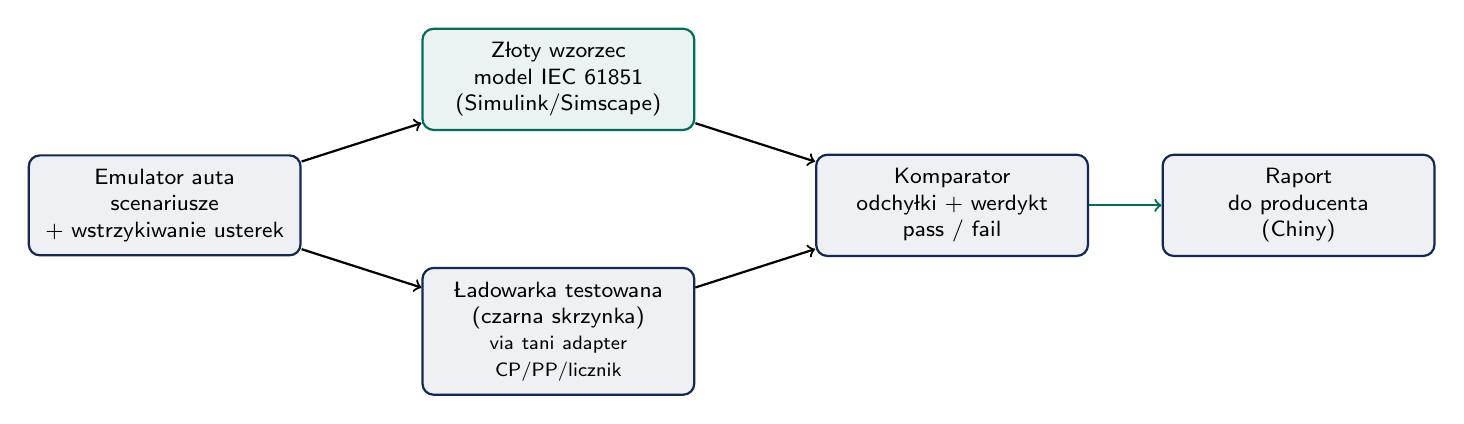
\begin{tikzpicture}[font=\sffamily\footnotesize,
  box/.style={draw=navy,thick,rounded corners,fill=navy!7,align=center,inner sep=5pt,text width=3.1cm,minimum height=1.15cm},
  gold/.style={draw=accent,thick,rounded corners,fill=accent!8,align=center,inner sep=5pt,text width=3.1cm,minimum height=1.15cm}]
  \node[box] (emul) at (0,0) {Emulator auta\\scenariusze\\+ wstrzykiwanie usterek};
  \node[gold] (g) at (5,1.6) {Złoty wzorzec\\model IEC 61851\\(Simulink/Simscape)};
  \node[box] (d) at (5,-1.6) {Ładowarka testowana\\(czarna skrzynka)\\{\scriptsize via tani adapter CP/PP/licznik}};
  \node[box] (c) at (10,0) {Komparator\\odchyłki + werdykt\\pass / fail};
  \node[box] (r) at (14.4,0) {Raport\\do producenta\\(Chiny)};
  \draw[->,thick] (emul) -- (g);
  \draw[->,thick] (emul) -- (d);
  \draw[->,thick] (g) -- (c);
  \draw[->,thick] (d) -- (c);
  \draw[->,thick,accent] (c) -- (r);
\end{tikzpicture}}
\end{center}

\subsection{Czym to się różni od ich obecnego „testera wallboxów''}

Obecny gadżet odpowiada na pytanie \key{„czy w ogóle działa?''} (go/no-go). Mój testbench odpowiada na \key{„jak dokładnie się zachowuje, gdzie odbiega od normy, o ile, i czy nowy firmware tego nie zepsuł?''} --- czyli charakteryzacja, regresja i materiał dowodowy dla producenta.

% ====== SYMULACJA ======
\section{4. Co dokładnie symuluję (Simulink/Simscape) --- i wolne alternatywy}

\subsection{Rdzeń modelu}
\begin{itemize}
  \item \key{Simscape Electrical --- analogowy front-end CP.} Źródło $\pm$12~V/PWM, sieć rezystorów auta (2,74~k$\Omega$ + dioda, dołączany 1,3~k$\Omega$), dzielnik. Widzę realne poziomy 12/9/6~V i kształt PWM --- dowód, że rozumiem warstwę fizyczną, nie tylko logikę.
  \item \key{Stateflow --- maszyna stanów CP.} Dwie sztuki: złoty wzorzec (ładowarka) i emulator auta. Pełen handshake A\ra{}B\ra{}C i z powrotem, z czasami przejść.
  \item \key{Logika prąd/PP.} Przeliczenie wypełnienie~\ra{}~prąd (\,$\times$0,6\,), kodowanie PP, wartości „raportowane'' jak w aplikacji.
\end{itemize}

\subsection{Scenariusz A (kluczowy): weryfikacja licznika energii}
Zadaję znany profil prądu w sesji, liczę \key{prawdziwą energię} (całka mocy po czasie), a model licznika obarczam konfigurowalnym błędem (offset, dryf, kwantyzacja). Testbench wykrywa, gdy \key{raportowane kWh} odbiega ponad tolerancję (np. $\pm$1\%). Efekt: zanim sprzęt trafi do floty, wiem, że licznik nie zawyża faktur --- a jeśli zawyża, mam dokładną liczbę do producenta.

\subsection{Scenariusz B (pokaz integracji): DLB}
Modeluję dom: bezpiecznik główny + zmienne obciążenie domowe + 1--4 ładowarki z DLB. Podnoszę obciążenie i sprawdzam, czy suma prądów \key{nigdy nie przekracza} bezpiecznika i czy ładowarka zdążyła zmniejszyć prąd w wymaganym czasie. Odpinam auto i sprawdzam, czy pozostałe „dobierają'' zwolnioną moc. To wprost dotyka realnych skarg: wybity bezpiecznik / wolne ładowanie.

\subsection{Wolne alternatywy (gdyby brak MATLAB-a)}
\key{Python} (NumPy/SciPy + prosta maszyna stanów, np.\ \texttt{transitions}) do logiki i scenariuszy; \key{Scilab/Xcos} jako darmowy odpowiednik Simulinka; \key{LTspice / ngspice / Falstad} do analogowego obwodu CP. Koncepcja jest niezależna od narzędzia --- MATLAB (licencja uczelniana) tylko ją przyspiesza.

% ====== PLAN 40H ======
\section{5. Plan pracy na ok. 40 h}

\begin{center}
\begin{tabularx}{\linewidth}{@{}c X c@{}}
\toprule
\textbf{Faza} & \textbf{Zakres} & \textbf{h} \\
\midrule
0 & Research normy IEC 61851 (CP/PP, czasy) + lista przypadków testowych & 4 \\
1 & Simscape: analogowy front-end CP (poziomy 12/9/6~V, PWM) & 6 \\
2 & Stateflow: maszyna stanów --- złoty wzorzec + emulator auta & 8 \\
3 & Logika wypełnienie\,\ra\,prąd + kodowanie PP + wartości raportowane & 3 \\
4 & Wstrzykiwanie usterek + komparator + werdykt pass/fail & 7 \\
5 & Scenariusz A: weryfikacja licznika energii (błąd kWh) & 5 \\
6 & Scenariusz B: DLB (bezpiecznik + obciążenia + 2--4 ładowarki) --- elastyczny & 4 \\
7 & Generator raportu do producenta + demo + opis koncepcji & 5 \\
\midrule
\multicolumn{2}{@{}r}{\textbf{Razem}} & \textbf{ok. 42} \\
\bottomrule
\end{tabularx}
\end{center}

Twardy rdzeń (fazy 0--5, 7) to ok. 38~h --- mieści się w budżecie nawet bez fazy DLB. Faza 6 jest „buforem jakości'': robię, jeśli rdzeń idzie sprawnie.

% ====== WARTOSC ======
\section{6. Co to realnie wyłapie (wartość diagnostyczna)}

Każdy przypadek to gotowy, odtwarzalny wpis do raportu dla producenta:

\begin{itemize}
  \item \key{Licznik zawyża/zaniża kWh} ponad tolerancję \ra{} złe rozliczenia floty (uderza w ich główny argument B2B).
  \item \key{Złe wypełnienie PWM} \ra{} ładowarka oferuje inny prąd, niż powinna (za wolno albo ponad bezpiecznik).
  \item \key{Brak reakcji na usterkę} (brak diody, zwarcie CP) zamiast odcięcia \ra{} problem bezpieczeństwa.
  \item \key{Za wolna reakcja DLB} ($>$ wymóg normy) \ra{} ryzyko wybicia bezpiecznika u klienta.
  \item \key{Regresja po nowym firmware:} przypadek, który wcześniej przechodził, teraz nie \ra{} złapane \key{przed} wysyłką do klientów.
\end{itemize}

Zamiast „klient mówi, że coś nie działa'' producent dostaje: \key{który scenariusz, jaka odchyłka, o ile, jak odtworzyć}. To realnie skraca pętlę poprawek z chińską fabryką.

% ====== BUDZET ======
\section{7. Budżet --- kapitał bliski zera}

\begin{center}
\begin{tabularx}{\linewidth}{@{}X r@{}}
\toprule
\textbf{Pozycja} & \textbf{Koszt} \\
\midrule
Symulacja: MATLAB/Simulink/Simscape (licencja uczelniana) & 0 zł \\
\;\; albo wariant darmowy: Python + Scilab/Xcos + LTspice & 0 zł \\
Czas: ok. 40~h pracy własnej & wkład własny \\
\midrule
\multicolumn{2}{@{}l}{\textit{Opcjonalnie --- dopiero do testów realnej ładowarki:}} \\
Tani adapter CP/PP + pomiar (MCU + analog) & 300--500 zł \\
Ładowarka do testów & sprzęt firmy \\
\midrule
\textbf{Koncept + symulacja (deliverable na poniedziałek)} & \textbf{ok. 0 zł kapitału} \\
\bottomrule
\end{tabularx}
\end{center}

To wprost odpowiada na ich strategię „nie topić kapitału'': najpierw tani model, dopiero potem ewentualny sprzęt.

% ====== RYZYKA ======
\section{8. Ryzyka i ograniczenia (uczciwie)}

\begin{itemize}
  \item \key{Model jest tak dobry, jak norma, którą koduję} --- dlatego faza 0 (rzetelne wczytanie IEC 61851) jest krytyczna.
  \item \key{Czarna skrzynka} --- niektóre zachowania wnioskuję z zewnątrz; testbench wskazuje \emph{co} odbiega, nie zawsze \emph{dlaczego} (to już rola producenta).
  \item \key{Adapter dotyka napięcia sieci} --- dlatego wersja symulacyjna jest pełnoprawnym deliverable, a sprzęt to osobny krok z zabezpieczeniami.
  \item \key{To nie certyfikacja} --- narzędzie wspiera diagnostykę i QA, nie zastępuje akredytowanych badań bezpieczeństwa.
\end{itemize}

% ====== PITCH ======
\section{9. Dlaczego to pasuje do firmy (pitch)}

AMPERE POINT zarabia na tym, że \key{lepiej testuje i szybciej adaptuje} cudzy sprzęt niż konkurencja --- „OEM na sterydach''. Mój projekt zamienia ich pętlę „testuj \ra{} zbierz feedback \ra{} zgłoś producentowi'' w \key{powtarzalny, tani, mierzalny proces}: złoty wzorzec łapie odchyłki, regresja pilnuje nowych firmware'ów, a weryfikacja licznika chroni ich główny argument dla flot. Zero kapitału na start, pełna symulacja jako dowód koncepcji --- i jasna ścieżka do wersji sprzętowej, gdy się opłaci.

\end{document}
